\section{System Description}
GIRAF is a collection of fully and partially interdependent applications for the Android platform, designed for use by children with Autism Spectrum Disorder.\newline
GIRAF consists of 5 projects with various degree of interaction. These projects are named Savannah, Oasis, GIRAF-Launcher, PARROT and WOMBAT. Each of these projects have produced individual products, which are parts of a greater project, GIRAF.\newline

\textbf{Savannah:} Savannah is a server designed for use with the GIRAF system. The server is meant to be available for users of GIRAF, and gives the functionality of data handling. For instance, Savannah will store all the data for a given department, making it available for everyone in the department to use on their Android tablet with GIRAF.\newline

\textbf{Oasis:} Oasis is an extra layer of functionality provided by the GIRAF project. It provides the Android tableet with a database for storing data, as well as functionality for syncronizing the database with that of the Savannah server, if it is available.\newline

\textbf{GIRAF-Launcher:} The GIRAF-Launcher is the main platform for GIRAF. It handles execution of GIRAF apps, and at the same time it provides safety features to ensure that a user that is not authorized to interact with the rest of the system will not be able to do so. When the launcher executes an app, it will provide it with profile information, specifying which child is currently using the app, as well as which guardian has signed in.\newline

\textbf{PARROT:} PARROT is an application for the GIRAF platform meant as a digital version of the pictures used for communication. PARROT provides the user with access to all his pictograms (meaning pictures with associated information such as sound and text), which can be used for communication. PARROT also gives guardians functionality for adding aditional pictograms, as well as organizing the pictograms into categories for ease of access, based on the needs of the individual child.\newline

\textbf{WOMBAT:} WOMBAT is an application for the GIRAF platform. Its purpose is to help the children to understand the aspect of time, by visualising it. WOMBAT provides many different ways of displaying time, as well as the possiblity to configure the app for the needs of the individual child. Such features include chosing between different representations of time, such as hour glasses and progress bars, as well as choosing the colour of them.\newline

\begin{figure}
	\centering
		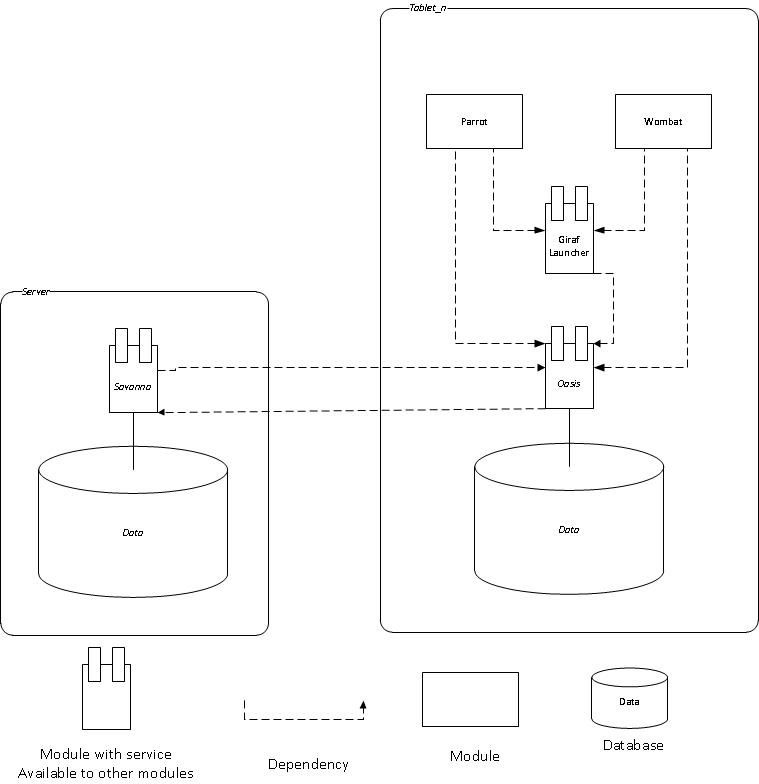
\includegraphics{.../common_report/images/Giraf_comp_pic.jpg}
	\caption{Component Structure of the Giraf Multiproject}
	\label{fig:Giraf_comp_pic}
\end{figure}
